\documentclass[12pt,a4paper]{article}
        \usepackage{graphicx}
        \usepackage{geometry}
        \geometry{margin=2cm}
        \usepackage{helvet}
        \usepackage{xcolor}
        \usepackage{amsmath} % for bmatrix
        \setlength{\parindent}{0pt}  % No indentation globally
        \renewcommand{\familydefault}{\sfdefault}
        \usepackage[german]{babel}% for glqq / grqq

        \begin{document}\begin{center}
                \Huge \textbf{Chlorobenzene} \\[1cm]
                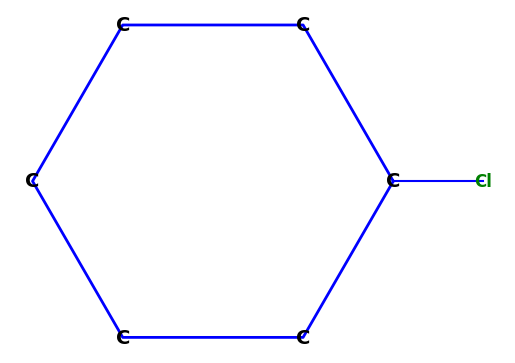
\includegraphics[width=0.5\textwidth]{chlorobenzene} \\[0.5cm]
                \Large Point Group: \textbf{C2v}
            \end{center}\newpage\section*{p orbitals}
Symmetry behavior of the p-orbitals:
$$\Gamma_{red} = \,7 E\;\oplus{}\,-3 C2\;\oplus{}\,-7 \sigma v(xz)\;\oplus{}\,3 \sigma v(yz)\;$$
$$\Gamma_{irred} = \,2 A2\;\oplus{}\,5 B2\;$$


\begin{itemize}
\item SALC of B2: \quad $p_{1}$
\item SALC of A2: \quad $\frac{\sqrt{2} p_{2}}{2} - \frac{\sqrt{2} p_{6}}{2}$
\item SALC of B2: \quad $\frac{\sqrt{2} p_{2}}{2} + \frac{\sqrt{2} p_{6}}{2}$
\item SALC of A2: \quad $\frac{\sqrt{2} p_{3}}{2} - \frac{\sqrt{2} p_{5}}{2}$
\item SALC of B2: \quad $\frac{\sqrt{2} p_{3}}{2} + \frac{\sqrt{2} p_{5}}{2}$
\item SALC of B2: \quad $p_{4}$
\item SALC of B2: \quad $p_{7}$
\end{itemize}
Put together these SALCs form the following Hamilton matrices:
     $$ H_{B2}= \left[\begin{bmatrix}\alpha & \sqrt{2} \beta & 0 & 0 & \beta_{Cl}\\\sqrt{2} \beta & \alpha & \beta & 0 & 0\\0 & \beta & \alpha & \sqrt{2} \beta & 0\\0 & 0 & \sqrt{2} \beta & \alpha & 0\\\beta_{Cl} & 0 & 0 & 0 & \alpha_{Cl}\end{bmatrix}\right]$$ 
     $$ H_{A2}= \left[\begin{bmatrix}\alpha & \beta\\\beta & \alpha\end{bmatrix}\right]$$ 


Solving Hückels secular equations, that follow from these H, leads to:
\begin{itemize}
\item orbital of A2 with energy = $\alpha + \beta$
\item orbital of A2 with energy = $\alpha - \beta$
\end{itemize}



\newpage \section*{s orbitals}
Symmetry behavior of the s-orbitals:
$$\Gamma_{red} = \,7 E\;\oplus{}\,3 C2\;\oplus{}\,7 \sigma v(xz)\;\oplus{}\,3 \sigma v(yz)\;$$
$$\Gamma_{irred} = \,5 A1\;\oplus{}\,2 B1\;$$


\begin{itemize}
\item SALC of A1: \quad $s_{1}$
\item SALC of A1: \quad $\frac{\sqrt{2} s_{2}}{2} + \frac{\sqrt{2} s_{6}}{2}$
\item SALC of B1: \quad $\frac{\sqrt{2} s_{2}}{2} - \frac{\sqrt{2} s_{6}}{2}$
\item SALC of A1: \quad $\frac{\sqrt{2} s_{3}}{2} + \frac{\sqrt{2} s_{5}}{2}$
\item SALC of B1: \quad $\frac{\sqrt{2} s_{3}}{2} - \frac{\sqrt{2} s_{5}}{2}$
\item SALC of A1: \quad $s_{4}$
\item SALC of A1: \quad $s_{7}$
\end{itemize}
Put together these SALCs form the following Hamilton matrices:
     $$ H_{A1}= \left[\begin{bmatrix}\alpha_{s} & \sqrt{2} \beta_{s} & 0 & 0 & \beta_{s Cl}\\\sqrt{2} \beta_{s} & \alpha_{s} & \beta_{s} & 0 & 0\\0 & \beta_{s} & \alpha_{s} & \sqrt{2} \beta_{s} & 0\\0 & 0 & \sqrt{2} \beta_{s} & \alpha_{s} & 0\\\beta_{s Cl} & 0 & 0 & 0 & \alpha_{s Cl}\end{bmatrix}\right]$$ 
     $$ H_{B1}= \left[\begin{bmatrix}\alpha_{s} & \beta_{s}\\\beta_{s} & \alpha_{s}\end{bmatrix}\right]$$ 


Solving Hückels secular equations, that follow from these H, leads to:
\begin{itemize}
\item orbital of B1 with energy = $\alpha_{s} + \beta_{s}$
\item orbital of B1 with energy = $\alpha_{s} - \beta_{s}$
\end{itemize}



\newpage \section*{Transitions from p orbitals into s orbitals}\subsection*{State with Occupation [2, 2, 2, 0, 0, 0, 2] (0 unpaired electrons, mult 1.0)}
        \noindent\textbf{Transition from $\phi_{2}$ into $\phi_{s_{2}}$:}
        \begin{itemize}
            \item $- [2, 2, 2, 0, 0, 0, 2], (0, 0, 0, 0, 0, 0, 0) \rightarrow (2, 1, 2, 0, 0, 0, 2), (0, 1, 0, 0, 0, 0, 0)$
        
            \item $\phi_{2}:$ linear combination = $- \sqrt{2} \left(\frac{\sqrt{2} p_{2}}{2} - \frac{\sqrt{2} p_{6}}{2}\right)$, \
            energy = $\alpha - \beta$
            
            \item $\xi_{2}:$ linear combination = $- \sqrt{2} \left(\frac{\sqrt{2} s_{2}}{2} - \frac{\sqrt{2} s_{6}}{2}\right)$, \
            energy = $\alpha_{s} - \beta_{s}$
            
            \item $\Delta$ Energy: $- \alpha + \alpha_{s} + \beta - \beta_{s}$
            \item Energy of State before Excitation: $4 \alpha$
            \item Energy of State after Excitation: $3 \alpha + \alpha_{s} + \beta - \beta_{s}$
            \item Energy between Average Energies of $\phi$-/$\xi$-orbitals: \
            $- \alpha + \alpha_{s}$
        
            \item dipole transition moment: $\delta$
        
        \end{itemize}
        
	\textcolor{red}{CAUTION:} state should have same length as occupation $\rightarrow$ missing results?
	DONT TRUST \glqq{}Energy of State before Excitation\grqq{}, only relative values are correct

\subsection*{State with Occupation (2, 1, 1, 1, 1, 0, 2) (4 unpaired electrons, mult 5.0)}
        \noindent\textbf{Transition from $\phi_{2}$ into $\phi_{s_{2}}$:}
        \begin{itemize}
            \item $- (2, 1, 1, 1, 1, 0, 2), (0, 0, 0, 0, 0, 0, 0) \rightarrow (2, 0, 1, 1, 1, 0, 2), (0, 1, 0, 0, 0, 0, 0)$
        
            \item $\phi_{2}:$ linear combination = $- \sqrt{2} \left(\frac{\sqrt{2} p_{2}}{2} - \frac{\sqrt{2} p_{6}}{2}\right)$, \
            energy = $\alpha - \beta$
            
            \item $\xi_{2}:$ linear combination = $- \sqrt{2} \left(\frac{\sqrt{2} s_{2}}{2} - \frac{\sqrt{2} s_{6}}{2}\right)$, \
            energy = $\alpha_{s} - \beta_{s}$
            
            \item $\Delta$ Energy: $- \alpha + \alpha_{s} + \beta - \beta_{s}$
            \item Energy of State before Excitation: $3 \alpha + \beta$
            \item Energy of State after Excitation: $2 \alpha + \alpha_{s} + 2 \beta - \beta_{s}$
            \item Energy between Average Energies of $\phi$-/$\xi$-orbitals: \
            $- \alpha + \alpha_{s}$
        
            \item dipole transition moment: $\delta$
        
        \end{itemize}
        
	\textcolor{red}{CAUTION:} state should have same length as occupation $\rightarrow$ missing results?
	DONT TRUST \glqq{}Energy of State before Excitation\grqq{}, only relative values are correct

\subsection*{State with Occupation (2, 1, 2, 0, 1, 0, 2) (2 unpaired electrons, mult 3.0)}
        \noindent\textbf{Transition from $\phi_{2}$ into $\phi_{s_{2}}$:}
        \begin{itemize}
            \item $- (2, 1, 2, 0, 1, 0, 2), (0, 0, 0, 0, 0, 0, 0) \rightarrow (2, 0, 2, 0, 1, 0, 2), (0, 1, 0, 0, 0, 0, 0)$
        
            \item $\phi_{2}:$ linear combination = $- \sqrt{2} \left(\frac{\sqrt{2} p_{2}}{2} - \frac{\sqrt{2} p_{6}}{2}\right)$, \
            energy = $\alpha - \beta$
            
            \item $\xi_{2}:$ linear combination = $- \sqrt{2} \left(\frac{\sqrt{2} s_{2}}{2} - \frac{\sqrt{2} s_{6}}{2}\right)$, \
            energy = $\alpha_{s} - \beta_{s}$
            
            \item $\Delta$ Energy: $- \alpha + \alpha_{s} + \beta - \beta_{s}$
            \item Energy of State before Excitation: $3 \alpha + \beta$
            \item Energy of State after Excitation: $2 \alpha + \alpha_{s} + 2 \beta - \beta_{s}$
            \item Energy between Average Energies of $\phi$-/$\xi$-orbitals: \
            $- \alpha + \alpha_{s}$
        
            \item dipole transition moment: $\delta$
        
        \end{itemize}
        
	\textcolor{red}{CAUTION:} state should have same length as occupation $\rightarrow$ missing results?
	DONT TRUST \glqq{}Energy of State before Excitation\grqq{}, only relative values are correct

\subsection*{State with Occupation (2, 1, 2, 1, 0, 0, 2) (2 unpaired electrons, mult 3.0)}
        \noindent\textbf{Transition from $\phi_{2}$ into $\phi_{s_{2}}$:}
        \begin{itemize}
            \item $- (2, 1, 2, 1, 0, 0, 2), (0, 0, 0, 0, 0, 0, 0) \rightarrow (2, 0, 2, 1, 0, 0, 2), (0, 1, 0, 0, 0, 0, 0)$
        
            \item $\phi_{2}:$ linear combination = $- \sqrt{2} \left(\frac{\sqrt{2} p_{2}}{2} - \frac{\sqrt{2} p_{6}}{2}\right)$, \
            energy = $\alpha - \beta$
            
            \item $\xi_{2}:$ linear combination = $- \sqrt{2} \left(\frac{\sqrt{2} s_{2}}{2} - \frac{\sqrt{2} s_{6}}{2}\right)$, \
            energy = $\alpha_{s} - \beta_{s}$
            
            \item $\Delta$ Energy: $- \alpha + \alpha_{s} + \beta - \beta_{s}$
            \item Energy of State before Excitation: $3 \alpha + \beta$
            \item Energy of State after Excitation: $2 \alpha + \alpha_{s} + 2 \beta - \beta_{s}$
            \item Energy between Average Energies of $\phi$-/$\xi$-orbitals: \
            $- \alpha + \alpha_{s}$
        
            \item dipole transition moment: $\delta$
        
        \end{itemize}
        
	\textcolor{red}{CAUTION:} state should have same length as occupation $\rightarrow$ missing results?
	DONT TRUST \glqq{}Energy of State before Excitation\grqq{}, only relative values are correct

\subsection*{State with Occupation (2, 2, 1, 0, 1, 0, 2) (2 unpaired electrons, mult 3.0)}
        \noindent\textbf{Transition from $\phi_{2}$ into $\phi_{s_{2}}$:}
        \begin{itemize}
            \item $- (2, 2, 1, 0, 1, 0, 2), (0, 0, 0, 0, 0, 0, 0) \rightarrow (2, 1, 1, 0, 1, 0, 2), (0, 1, 0, 0, 0, 0, 0)$
        
            \item $\phi_{2}:$ linear combination = $- \sqrt{2} \left(\frac{\sqrt{2} p_{2}}{2} - \frac{\sqrt{2} p_{6}}{2}\right)$, \
            energy = $\alpha - \beta$
            
            \item $\xi_{2}:$ linear combination = $- \sqrt{2} \left(\frac{\sqrt{2} s_{2}}{2} - \frac{\sqrt{2} s_{6}}{2}\right)$, \
            energy = $\alpha_{s} - \beta_{s}$
            
            \item $\Delta$ Energy: $- \alpha + \alpha_{s} + \beta - \beta_{s}$
            \item Energy of State before Excitation: $4 \alpha$
            \item Energy of State after Excitation: $3 \alpha + \alpha_{s} + \beta - \beta_{s}$
            \item Energy between Average Energies of $\phi$-/$\xi$-orbitals: \
            $- \alpha + \alpha_{s}$
        
            \item dipole transition moment: $\delta$
        
        \end{itemize}
        
	\textcolor{red}{CAUTION:} state should have same length as occupation $\rightarrow$ missing results?
	DONT TRUST \glqq{}Energy of State before Excitation\grqq{}, only relative values are correct

\subsection*{State with Occupation (2, 2, 1, 1, 0, 0, 2) (2 unpaired electrons, mult 3.0)}
        \noindent\textbf{Transition from $\phi_{2}$ into $\phi_{s_{2}}$:}
        \begin{itemize}
            \item $- (2, 2, 1, 1, 0, 0, 2), (0, 0, 0, 0, 0, 0, 0) \rightarrow (2, 1, 1, 1, 0, 0, 2), (0, 1, 0, 0, 0, 0, 0)$
        
            \item $\phi_{2}:$ linear combination = $- \sqrt{2} \left(\frac{\sqrt{2} p_{2}}{2} - \frac{\sqrt{2} p_{6}}{2}\right)$, \
            energy = $\alpha - \beta$
            
            \item $\xi_{2}:$ linear combination = $- \sqrt{2} \left(\frac{\sqrt{2} s_{2}}{2} - \frac{\sqrt{2} s_{6}}{2}\right)$, \
            energy = $\alpha_{s} - \beta_{s}$
            
            \item $\Delta$ Energy: $- \alpha + \alpha_{s} + \beta - \beta_{s}$
            \item Energy of State before Excitation: $4 \alpha$
            \item Energy of State after Excitation: $3 \alpha + \alpha_{s} + \beta - \beta_{s}$
            \item Energy between Average Energies of $\phi$-/$\xi$-orbitals: \
            $- \alpha + \alpha_{s}$
        
            \item dipole transition moment: $\delta$
        
        \end{itemize}
        
	\textcolor{red}{CAUTION:} state should have same length as occupation $\rightarrow$ missing results?
	DONT TRUST \glqq{}Energy of State before Excitation\grqq{}, only relative values are correct

\newpage \section*{Dispersion energies following from the transitions}

\begin{enumerate}
 \item State: A = [2, 2, 2, 0, 0, 0, 2] $\leftrightarrow$ B = (2, 1, 1, 1, 1, 0, 2) 
$$E_{dispersion} =\frac{8 \delta^{4}}{r^{6} \left(- 2 \alpha + 2 \alpha_{s} + 2 \beta - 2 \beta_{s}\right)}$$
 \item State: A = (2, 1, 1, 1, 1, 0, 2) $\leftrightarrow$ B = [2, 2, 2, 0, 0, 0, 2] 
$$E_{dispersion} =\frac{8 \delta^{4}}{r^{6} \left(- 2 \alpha + 2 \alpha_{s} + 2 \beta - 2 \beta_{s}\right)}$$
 \item State: A = (2, 1, 2, 0, 1, 0, 2) $\leftrightarrow$ B = (2, 1, 2, 0, 1, 0, 2) 
$$E_{dispersion} =\frac{4 \delta^{4}}{r^{6} \left(- 2 \alpha + 2 \alpha_{s} + 2 \beta - 2 \beta_{s}\right)}$$
 \item State: A = (2, 1, 2, 0, 1, 0, 2) $\leftrightarrow$ B = (2, 1, 2, 1, 0, 0, 2) 
$$E_{dispersion} =\frac{4 \delta^{4}}{r^{6} \left(- 2 \alpha + 2 \alpha_{s} + 2 \beta - 2 \beta_{s}\right)}$$
 \item State: A = (2, 1, 2, 0, 1, 0, 2) $\leftrightarrow$ B = (2, 2, 1, 0, 1, 0, 2) 
$$E_{dispersion} =\frac{8 \delta^{4}}{r^{6} \left(- 2 \alpha + 2 \alpha_{s} + 2 \beta - 2 \beta_{s}\right)}$$
 \item State: A = (2, 1, 2, 0, 1, 0, 2) $\leftrightarrow$ B = (2, 2, 1, 1, 0, 0, 2) 
$$E_{dispersion} =\frac{8 \delta^{4}}{r^{6} \left(- 2 \alpha + 2 \alpha_{s} + 2 \beta - 2 \beta_{s}\right)}$$
 \item State: A = (2, 1, 2, 1, 0, 0, 2) $\leftrightarrow$ B = (2, 1, 2, 0, 1, 0, 2) 
$$E_{dispersion} =\frac{4 \delta^{4}}{r^{6} \left(- 2 \alpha + 2 \alpha_{s} + 2 \beta - 2 \beta_{s}\right)}$$
 \item State: A = (2, 1, 2, 1, 0, 0, 2) $\leftrightarrow$ B = (2, 1, 2, 1, 0, 0, 2) 
$$E_{dispersion} =\frac{4 \delta^{4}}{r^{6} \left(- 2 \alpha + 2 \alpha_{s} + 2 \beta - 2 \beta_{s}\right)}$$
 \item State: A = (2, 1, 2, 1, 0, 0, 2) $\leftrightarrow$ B = (2, 2, 1, 0, 1, 0, 2) 
$$E_{dispersion} =\frac{8 \delta^{4}}{r^{6} \left(- 2 \alpha + 2 \alpha_{s} + 2 \beta - 2 \beta_{s}\right)}$$
 \item State: A = (2, 1, 2, 1, 0, 0, 2) $\leftrightarrow$ B = (2, 2, 1, 1, 0, 0, 2) 
$$E_{dispersion} =\frac{8 \delta^{4}}{r^{6} \left(- 2 \alpha + 2 \alpha_{s} + 2 \beta - 2 \beta_{s}\right)}$$
 \item State: A = (2, 2, 1, 0, 1, 0, 2) $\leftrightarrow$ B = (2, 1, 2, 0, 1, 0, 2) 
$$E_{dispersion} =\frac{8 \delta^{4}}{r^{6} \left(- 2 \alpha + 2 \alpha_{s} + 2 \beta - 2 \beta_{s}\right)}$$
 \item State: A = (2, 2, 1, 0, 1, 0, 2) $\leftrightarrow$ B = (2, 1, 2, 1, 0, 0, 2) 
$$E_{dispersion} =\frac{8 \delta^{4}}{r^{6} \left(- 2 \alpha + 2 \alpha_{s} + 2 \beta - 2 \beta_{s}\right)}$$
 \item State: A = (2, 2, 1, 0, 1, 0, 2) $\leftrightarrow$ B = (2, 2, 1, 0, 1, 0, 2) 
$$E_{dispersion} =\frac{16 \delta^{4}}{r^{6} \left(- 2 \alpha + 2 \alpha_{s} + 2 \beta - 2 \beta_{s}\right)}$$
 \item State: A = (2, 2, 1, 0, 1, 0, 2) $\leftrightarrow$ B = (2, 2, 1, 1, 0, 0, 2) 
$$E_{dispersion} =\frac{16 \delta^{4}}{r^{6} \left(- 2 \alpha + 2 \alpha_{s} + 2 \beta - 2 \beta_{s}\right)}$$
 \item State: A = (2, 2, 1, 1, 0, 0, 2) $\leftrightarrow$ B = (2, 1, 2, 0, 1, 0, 2) 
$$E_{dispersion} =\frac{8 \delta^{4}}{r^{6} \left(- 2 \alpha + 2 \alpha_{s} + 2 \beta - 2 \beta_{s}\right)}$$
 \item State: A = (2, 2, 1, 1, 0, 0, 2) $\leftrightarrow$ B = (2, 1, 2, 1, 0, 0, 2) 
$$E_{dispersion} =\frac{8 \delta^{4}}{r^{6} \left(- 2 \alpha + 2 \alpha_{s} + 2 \beta - 2 \beta_{s}\right)}$$
 \item State: A = (2, 2, 1, 1, 0, 0, 2) $\leftrightarrow$ B = (2, 2, 1, 0, 1, 0, 2) 
$$E_{dispersion} =\frac{16 \delta^{4}}{r^{6} \left(- 2 \alpha + 2 \alpha_{s} + 2 \beta - 2 \beta_{s}\right)}$$
 \item State: A = (2, 2, 1, 1, 0, 0, 2) $\leftrightarrow$ B = (2, 2, 1, 1, 0, 0, 2) 
$$E_{dispersion} =\frac{16 \delta^{4}}{r^{6} \left(- 2 \alpha + 2 \alpha_{s} + 2 \beta - 2 \beta_{s}\right)}$$
\end{enumerate}
Ground-State:

A =[2, 2, 2, 0, 0, 0, 2]$\leftrightarrow$ B =[2, 2, 2, 0, 0, 0, 2]
$$E_{dispersion} =- \frac{8 \delta^{4}}{r^{6} \left(\alpha - \alpha_{s} - \beta + \beta_{s}\right)}$$


\end{document}